\section{Calibration and Empirical Grounding}
\label{sec:calibration}

% BUDGET: 2,000 words of prose (SOL_PLAN_REFORMAT.md), of which roughly 250 are reserved
% for the results-dependent close of Section~\ref{sec:data-validation} (the BNPL-on
% independent checks and the explicit answer to RQ1), written after the final run.
% This section says where every number comes from, and keeps what is IMPOSED from data
% or literature strictly apart from what is ESTIMATED.

This section describes the data, parameter choices, calibration and validation checks.
Table~\ref{tab:param-taxonomy} separates observed, constructed, imported, fitted and assumed inputs.
Only two parameters are fitted; assumptions without empirical estimates are varied in sensitivity analysis.
Appendix~\ref{app:specification} gives the full parameter register.

\begin{table}[H]
\centering
\caption{Where the model's numbers come from}
\label{tab:param-taxonomy}
\tabnote{The five classes of model input, in descending order of empirical standing, with the principal members of each and where each is documented. ``Imported'' means estimated on a foreign population and applied to South African households without local evidence; ``swept'' means that no source fixes the value, so results are reported across a range and never at a single point. The parameter register (Table~\ref{tab:param-register}) records the class of every individual parameter.}
\begin{tabular}{L{2.2cm}L{6.9cm}L{4.3cm}}
\toprule
\textbf{Class} & \textbf{Principal members} & \textbf{Documented in} \\
\midrule
Observed & Household income, expenditure, savings and debt (\ac{NIDS} 2017); financial-inclusion flags (\acs{FinScope} 2019); statutory rate ceilings and the Regulation 23A expense table; \ac{BNPL} contract terms, order cap and late fees; the re-employment hazard (\ac{QLFS} 2017) & Sections~\ref{sec:population} and~\ref{sec:servicing}; Appendix~\ref{app:variables} \\
\addlinespace
Constructed & Scheduled debt service (amortised from stocks); income quintiles and reference groups; the purchase ratio $\kappa$ (IES 2022/23); 2017-Rand deflation of \ac{BNPL} money parameters & Section~\ref{sec:servicing}; Appendix~\ref{app:variables} \\
\addlinespace
Imported & Minimum-payer share of 0.29; the present-bias and social-approval evidence behind payment friction and want-driven borrowing (all United States) & Section~\ref{sec:lim-transfer} \\
\addlinespace
Fitted & Income-shock probability (to the \ac{CCMR} 90+ day band); payment-friction rate (to the 1--30 day band) & Section~\ref{sec:lim-calibration} \\
\addlinespace
Swept & Peer coefficients $q_{\text{base}}$, $\beta$ and the threshold parameters; the shortfall amount rule and its \ac{BNPL} cap; the minimum-payment fraction; the rolling limit $\lambda$ & Sections~\ref{sec:lim-calibration} and~\ref{sec:results-robustness} \\
\bottomrule
\end{tabular}
\end{table}

\subsection{Simulation Parameters}
\label{sec:sim-params}

Each run simulates 5{,}000 households for 52 ticks (approximately two years), with the first 12 ticks treated as initialisation burn-in for post-burn-in summaries.
Every configuration is replicated twenty times with seeds $s_0 + i$, where $s_0$ is fixed per experiment suite, so any single run can be reproduced from its reported seed, and dispersion across replicates is reported with every result.
Threshold endowments are drawn from a separate random stream, so control arms reproduce exactly and a sweep over threshold dispersion is a paired comparison.

\subsection{The Household Population}
\label{sec:population}

We construct a synthetic population of 5{,}000 household agents from South African microdata, with all monetary figures in 2017 South African Rand (ZAR), the base survey year, and no inflation adjustment at the data layer.

\subsubsection*{Primary Dataset: NIDS Wave 5}
\label{sec:backbone}

The backbone of the synthetic population is drawn from \ac{NIDS} Wave 5 \cite{nids_w5_2018}.
Filtering the raw sample ($N = 13,719$) for households with reported income, valid size, and
positive sampling weights leaves 10{,}841 records. The 2{,}878 discarded records carry zero or missing weights; their removal thus entails no loss of weighted population mass. Scaled by national design weights, the final sample represents 18.67 million households or roughly 56.5 million individuals.

We derive six core economic variables per household: monthly income and its dominant source (wage, grant, or remittance and other); committed expenditure (food and rent paid, an incompressible floor); discretionary expenditure (all other non-food cash spending); liquid savings (financial assets, winsorised at the 99th percentile); and traditional debt (outstanding financial debt).
Imputed rent, the non-cash consumption value of owner-occupied housing, is excluded from both expenditure tiers.
Asset, debt and rent fields that the survey records only for holders are set to zero where missing, a choice Section~\ref{sec:data-validation} tests against aggregate national credit data, and households are stratified into per-capita income quintiles.
Appendix~\ref{app:variables} gives the source field, formula, missing-data treatment and diagnostics for every variable, including the debt-service construction of Section~\ref{sec:servicing}.

\subsubsection*{Imputing Financial Inclusion: FinScope 2019}
\label{sec:match}

Because \ac{NIDS} omits institutional banking status and specific debt instruments, we impute six binary financial inclusion indicators from the 2019 \ac{FinScope} survey \cite{finscope2019}.
Banked status determines entry into \ac{BNPL}, bounding potential market adoption at the observed 82.8\% macro limit rather than an arbitrary baseline parameter.
Five credit-product flags (store cards, revolving credit, hire purchase, short-term loans, and personal loans) determine the interest rates and repayment schedules assigned in Section~\ref{sec:servicing}.

We transfer attributes using cell-donor matching, illustrated in Figure~\ref{fig:cell-donor}.
Stratifying both datasets by per-capita income quintile and province, each \ac{NIDS} record draws a donor from its matching cell with probability proportional to the donor's survey weight (seed: 42).
Each of the 45 sampling cells contains at least 30 donor candidates, and no draw ever fell back to a coarser cell.

Copying all six flags from one donor preserves observed combinations of product holdings and their weighted cell distribution in expectation.
The match retains variation within cells, but does not preserve associations between the flags and unmatched recipient characteristics, such as urban or rural location.
This may change where exposure concentrates.
The two-year vintage gap may also overstate banking access in the 2017 population.
Appendix~\ref{app:matching} details these assumptions and reports donor reuse.

\begin{figure}[H]
\centering
\begin{tikzpicture}[font=\footnotesize, >=Stealth,
  cell/.style={draw, minimum width=0.46cm, minimum height=0.34cm, inner sep=0pt},
  hl/.style={fill=black!18},
  rec/.style={draw, rounded corners=1pt, align=center, inner sep=4pt},
  donor/.style={circle, draw, fill=black!8, inner sep=0pt},
  lbl/.style={align=center}]
% ---- panel (a): the same partition of both surveys --------------------------
\node[lbl] at (-0.55,2.2) {\textbf{(a)}};
\foreach \x in {0,...,8} \foreach \y in {0,...,4} {
  \node[cell] at (\x*0.46, \y*0.34) {};
  \node[cell] at (6.7+\x*0.46, \y*0.34) {};
}
\node[cell, hl] (rcell) at (2*0.46, 3*0.34) {};
\node[cell, hl] (dcell) at (6.7+2*0.46, 3*0.34) {};
\foreach \y/\l in {0/Q1,1/Q2,2/Q3,3/Q4,4/Q5} {
  \node[left, font=\scriptsize] at (-0.28,\y*0.34) {\l};
  \node[left, font=\scriptsize] at (6.42,\y*0.34) {\l}; }
\node[lbl] at (1.85,-0.68) {\textbf{NIDS 2017}, 10{,}841 recipients\\[-2pt] \scriptsize nine provinces $\rightarrow$};
\node[lbl] at (8.55,-0.68) {\textbf{FinScope 2019}, 4{,}969 donors\\[-2pt] \scriptsize nine provinces $\rightarrow$};
\draw[->, thick] (rcell.north) to[out=75, in=105] node[midway, above, lbl]
  {the same cell $c = (q, p)$: 45 cells, each with at least 30 donors} (dcell.north);
% ---- panel (b): one donor, the whole vector ---------------------------------
\node[lbl] at (-0.55,-1.7) {\textbf{(b)}};
\node[rec] (recip) at (1.5,-2.9) {recipient $i$\\[1pt] \scriptsize income, expenditure,\\[-1pt] \scriptsize savings, debt from \ac{NIDS}};
\node[donor, minimum size=14pt, fill=black!40] (d3) at (8.55,-2.9) {};
\node[donor, minimum size=6pt]  (d6) at (8.9,-2.2) {};
\node[donor, minimum size=5pt]  (d1) at (9.45,-2.4) {};
\node[donor, minimum size=9pt]  (d2) at (10.05,-2.75) {};
\node[donor, minimum size=7pt]  (d4) at (10.55,-3.2) {};
\node[donor, minimum size=11pt] (d5) at (9.4,-3.4) {};
\node[draw, dashed, fit=(d1)(d2)(d3)(d4)(d5)(d6), inner sep=5pt,
  label={[lbl, font=\scriptsize, yshift=-2pt]below:donor pool of cell $c$;\\ circle area $\propto$ weight $w_d$}] (pool) {};
\draw[->, thick] (d3.west) -- (recip.east)
  node[midway, above, lbl, yshift=1pt] {one donor $d$, drawn with\\ probability $w_d / \sum_{d' \in c} w_{d'}$}
  node[midway, below, lbl, font=\scriptsize, yshift=-1pt] {copies the whole\\ six-flag vector};
% ---- panel (c): the rejected alternative ------------------------------------
\node[lbl] at (-0.55,-4.75) {\textbf{(c)}};
\node[rec] (recip2) at (1.5,-5.7) {recipient $i$\\[1pt] \scriptsize per-flag imputation\\[-1pt] \scriptsize (rejected)};
\foreach \k/\ypos in {1/-4.95,2/-5.25,3/-5.55,4/-5.85,5/-6.15,6/-6.45} {
  \node[donor, minimum size=6pt] (e\k) at (8.55,\ypos) {};
  \draw[->, thin] (e\k.west) -- (recip2.east); }
\node[lbl, right, font=\scriptsize] at (8.85,-5.7) {six draws from six\\ different donors: the same\\ marginals, but the joint\\ structure stacking depends\\ on is lost};
\end{tikzpicture}
\caption{The cell-donor match}
\label{fig:cell-donor}
\tabnote{Panel (a): both surveys are partitioned into the same 45 cells by per-capita income quintile and province; a \ac{NIDS} household draws its donor only from the \ac{FinScope} households in its own cell, and every cell holds at least 30 donors. Panel (b): within the cell, one donor is drawn with probability proportional to its survey weight (circle area), and its entire six-flag vector is copied to the recipient, so each recipient receives a combination observed in the donor survey. Panel (c): the rejected alternative, one draw per flag from six different donors, reproduces the same marginals but discards the joint structure that concurrent-facility stacking depends on. Appendix~\ref{app:matching} gives the procedure formally, with its assumptions and limits.}
\end{figure}

The imputed rates match their national targets to within 1.8 percentage points (Table~\ref{tab:imputation_errors}) and to within 2.3 across all thirty quintile-by-indicator cells (Figure~\ref{fig:inclusion-fidelity}).

\begin{table}[H]
\centering
\caption{National rates for the six imputed indicators}
\label{tab:imputation_errors}
\tabnote{This table compares the national rate of each imputed indicator in three populations: the \ac{FinScope} 2019 benchmark, weighted by its survey weight; the 10{,}841-household synthetic population after matching, weighted by \ac{NIDS} survey weight; and the unweighted 5{,}000-agent resample used in the simulation. The difference column is synthetic less \ac{FinScope}, in percentage points, computed before rounding; the tolerance is 3 percentage points (Table~\ref{tab:validation}). Because the match draws donors within the same quintile-by-province cell in proportion to weight, agreement here is expected by construction: it tests the implementation, not the population's external validity (Appendix~\ref{app:matching}).}
\begin{tabular}{lrrrr}
\toprule
\textbf{Imputed indicator} & \textbf{FinScope 2019} & \textbf{Synthetic} & \textbf{Agents} & \textbf{Difference} \\
 & \textbf{(\%)} & \textbf{(\%)} & \textbf{(\%)} & \textbf{(pp)} \\
\midrule
Banked status    & 82.4 & 82.8 & 82.8 & 0.4 \\
Store card       & 20.8 & 22.6 & 21.8 & 1.8 \\
Revolving credit &  3.7 &  4.1 &  3.8 & 0.5 \\
Hire purchase    &  6.5 &  6.9 &  6.5 & 0.5 \\
Short-term loan  &  2.7 &  3.4 &  3.3 & 0.6 \\
Personal loan    &  2.1 &  2.3 &  2.3 & 0.2 \\
\bottomrule
\end{tabular}
\end{table}

\begin{figure}[htbp]
\centering
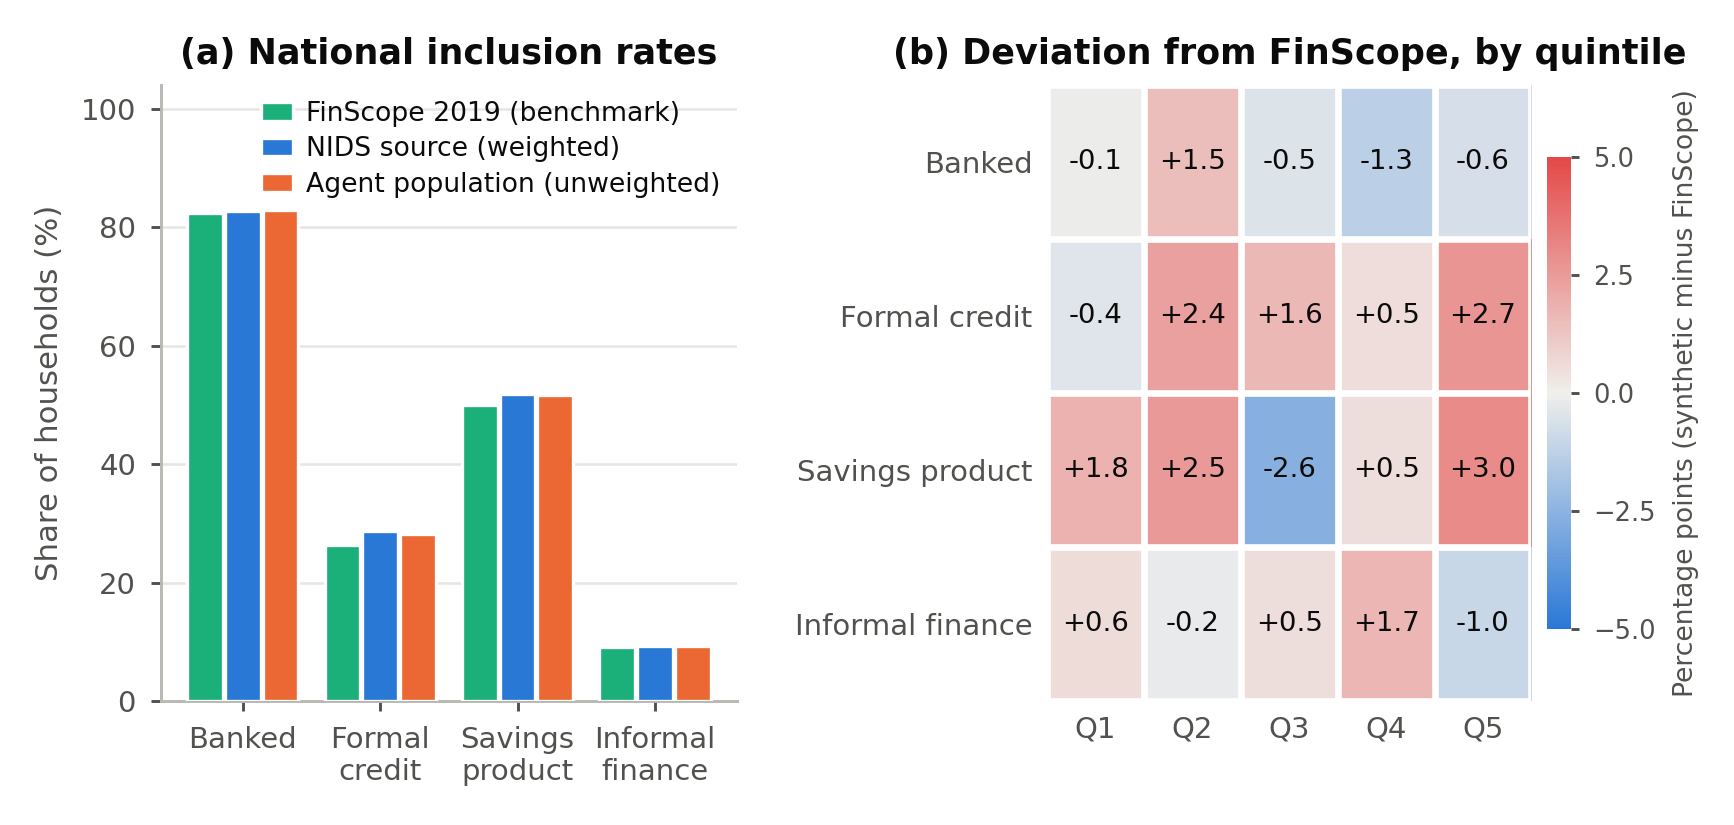
\includegraphics[width=\textwidth]{figures/fig_inclusion_fidelity.pdf}
\caption{Fidelity of the imputed indicators}
\label{fig:inclusion-fidelity}
\tabnote{Panel (a) compares the national rate of each of the six imputed indicators across the \ac{FinScope} 2019 benchmark, the weighted synthetic population and the unweighted 5{,}000-agent population, as in Table~\ref{tab:imputation_errors}. Panel (b) shows the synthetic-less-\ac{FinScope} gap for each indicator within each per-capita income quintile, thirty cells in all; the largest single deviation is 2.3 percentage points against a tolerance of 5. Quintiles are the weighted \ac{NIDS} bounds of Appendix~\ref{app:variables}.}
\end{figure}

\subsubsection*{Population Resampling}
\label{sec:resample}

The 10{,}841 weighted \ac{NIDS} households are resampled with replacement proportional to survey weights (seed: 20260818) to form a standard unweighted agent population of $N = 5{,}000$, so that downstream simulation statistics are calculated unweighted and reflect empirical distributional properties directly.
Figure~\ref{fig:pop-fidelity} illustrates structural alignment between the resampled agents and the weighted source data; resampling slightly increases concentration, the per-capita income Gini coefficient rising from 0.651 in the weighted sample to 0.667 in the agent population.

\begin{figure}[htbp]
\centering
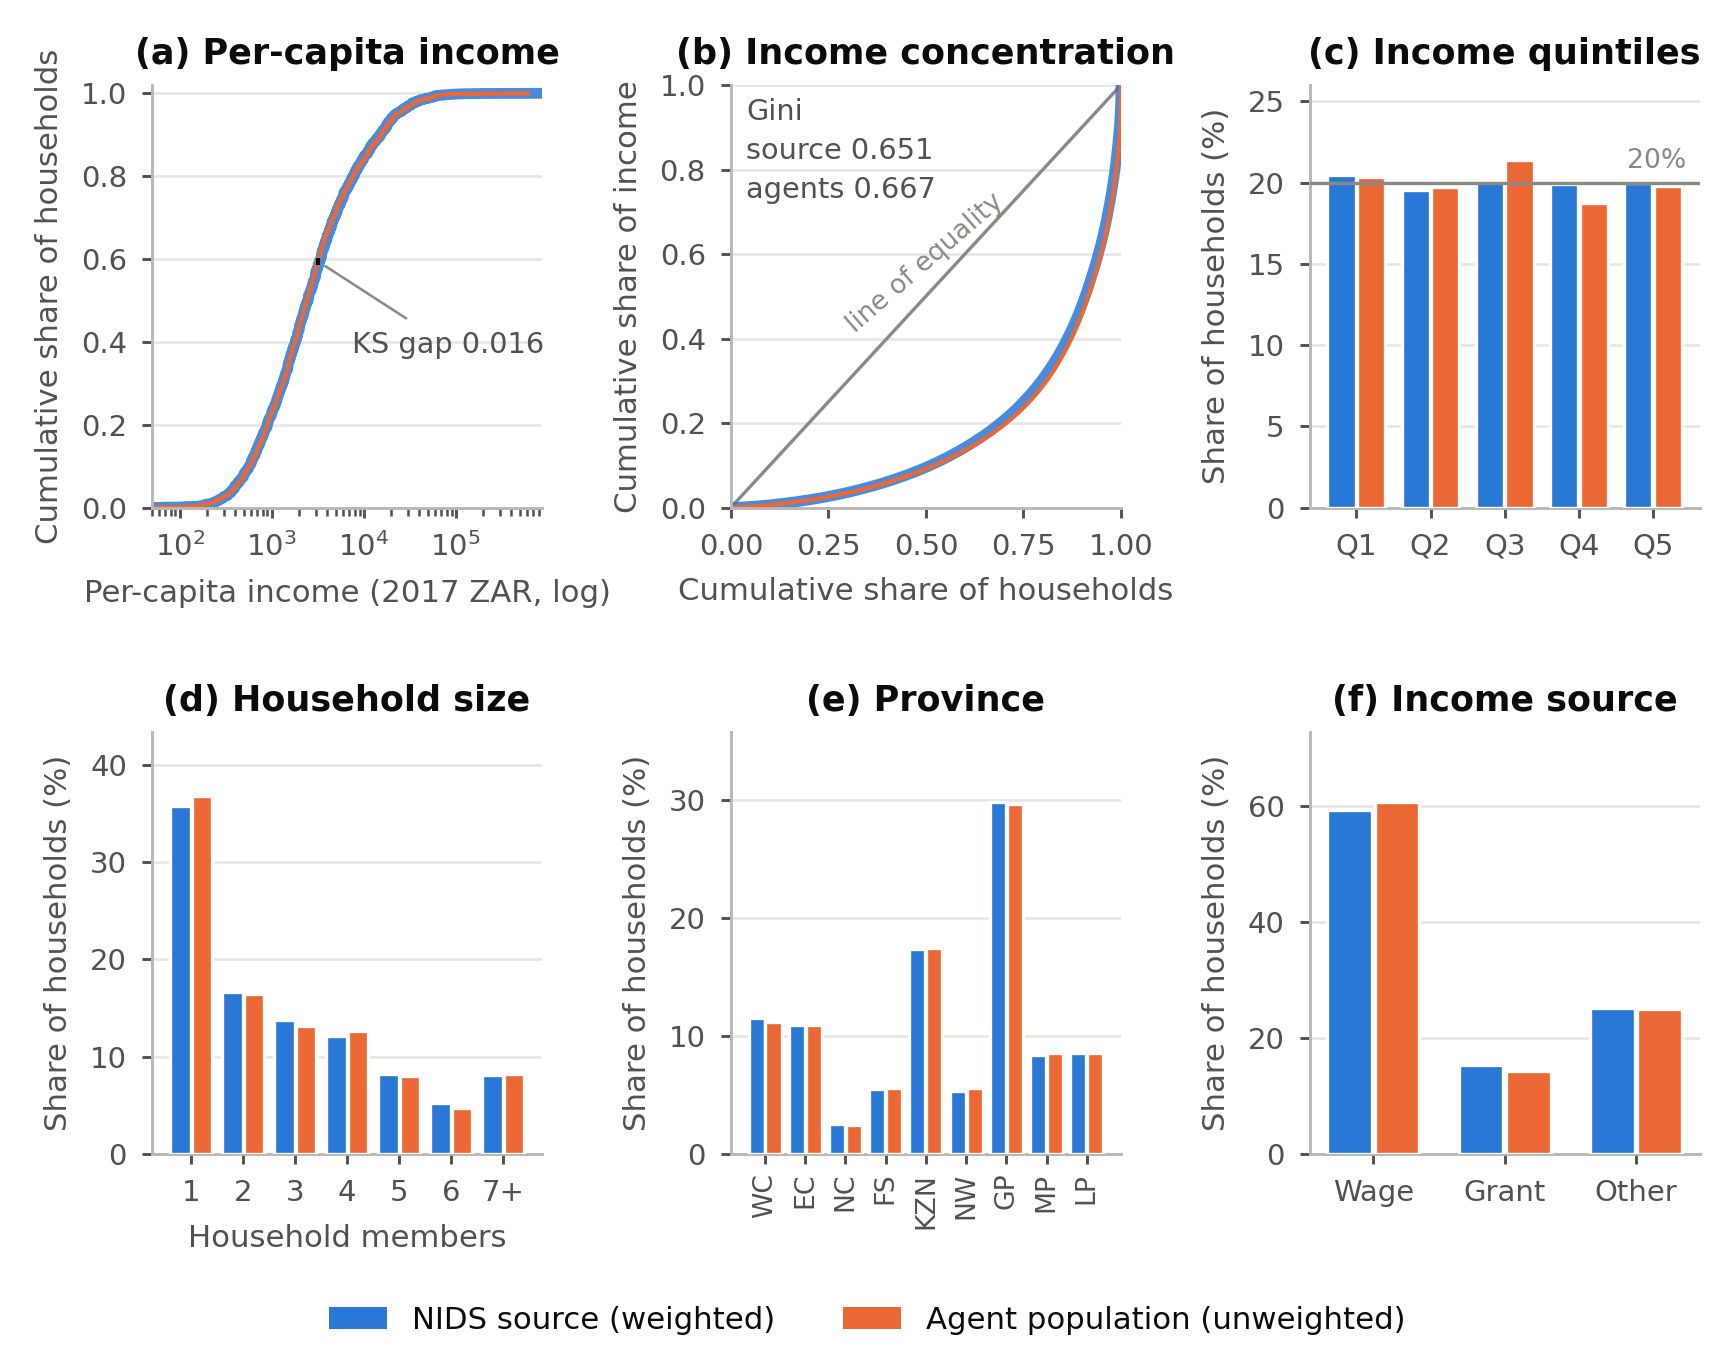
\includegraphics[width=\textwidth]{figures/fig_population_fidelity.pdf}
\caption{Distributional fidelity of the agent population}
\label{fig:pop-fidelity}
\tabnote{Each panel compares the unweighted 5{,}000-agent resample, drawn with replacement in proportion to \ac{NIDS} survey weight (seed 20260818) from 3{,}221 unique source records, against the weighted 10{,}841-household source it is drawn from. Panels (a) and (b) cover the per-capita income distribution and its concentration; panels (c) to (f) cover income quintile, household size, province and primary income source, the categorical attributes that gate behaviour and define the reference groups in the simulation. The Kolmogorov--Smirnov distance in (a) is 0.016, the largest categorical deviation across the 24 sub-categories is 1.4 percentage points, and the Gini rises from 0.651 to 0.667.}
\end{figure}

\subsection{Debt-Service and Product Parameters}
\label{sec:servicing}

\ac{NIDS} measures debt \emph{stocks}, but the simulation requires monthly cash \emph{flows}.
Monthly debt service is reconstructed in three steps, specified in full in Appendix~\ref{app:variables}: each household's balance is amortised at the \ac{NCA} statutory maximum \ac{APR} for 2017 \cite{sa_ncr_ratecaps_2016} over a product-specific repayment horizon (Table~\ref{tab:credit-terms}), and the resulting instalment is capped at the Regulation 23A residual-income ceiling \cite{sa_ncr_affordability_2015}.
Because realised rates by product class are unobserved in the \ac{CCMR} \cite{ncr_ccmr_2017} or any collateral 2017 source, statutory ceilings serve as proxies and bias calculated debt service upward.
Because \ac{NIDS} reports one consolidated balance, each household adopts the unweighted mean rate and horizon across the product classes its donor flags; balances with no flagged product are priced as unsecured.

\begin{table}[tbp]
\centering
\caption{Interest rates and repayment horizons by product class}
\label{tab:credit-terms}
\tabnote{This table gives the annual rate and repayment horizon used to amortise each household's opening traditional debt, by the product class its \ac{FinScope} donor flags; a household holding several classes takes the unweighted mean of each. Rates are the \ac{NCA} statutory maxima at the 2017 repurchase rate of 7.00\% \cite{sa_ncr_ratecaps_2016}, not realised market rates, which no 2017 source publishes; they therefore bound calculated debt service from above. Horizons are either measured in \ac{NIDS} as the median ratio of balance to the observed monthly payment for that product ($n$ as shown) or derived from the \ac{CCMR} stock-flow implied life, three times the gross debtors book over quarterly credit granted. Construction detail is in Appendix~\ref{app:variables}.}
\begin{tabular}{L{2.7cm}L{1.2cm}L{1.9cm}L{5.7cm}}
\toprule
\textbf{Product class} & \textbf{\ac{APR}} & \textbf{Horizon (months)} & \textbf{Provenance} \\
\midrule
Store card & 21\% & 11 & Measured in \ac{NIDS}: median balance over observed monthly clothing-account payment, $n=782$ \cite{nids_w5_2018} \\
\addlinespace
Hire purchase & 24\% & 8 & Measured in \ac{NIDS}: median balance over observed monthly hire-purchase payment, $n=121$ \cite{nids_w5_2018} \\
\addlinespace
Short-term loan & 60\% & 1 & \ac{FinScope} defines the product as repayable within 31 days; the \ac{CCMR} places 65.8\% of such agreements at one month or less \cite{finscope2019, ncr_ccmr_2017} \\
\addlinespace
Personal loan & 28\% & 25 & \ac{CCMR} stock-flow implied life of the unsecured book, 24.8 months \cite{ncr_ccmr_2017} \\
\addlinespace
Revolving credit & 21\% & 20 & No contractual term exists. Derived as the reciprocal of the mid-range minimum-payment fraction, which is swept over 0.025 to 0.10 \\
\addlinespace
Unflagged balance & 28\% & 25 & Fallback for the 74.0\% of donors flagging no specific product; mapped as personal loan \\
\bottomrule
\end{tabular}
\end{table}

The affordability cap binds for 3.8\% of indebted households but removes 22.8\% of total calculated debt service, so the adjustment is concentrated on high-debt outliers (Appendix~\ref{app:var-servicing}).
One accounting overlap is known: the \ac{NIDS} non-food aggregate already contains reported clothing-account, hire-purchase and vehicle payments (median 12.6\% of non-food outlay among households reporting one), so constructed servicing charges a flow partly present in discretionary spending, overstating compressible outlay for indebted agents and understating their relative servicing share.
These assumptions affect the level of simulated distress, but their combined effect does not establish an upper bound on default or on scenario differences.

The \ac{BNPL} product is parameterised from what providers publish: contract structure, the per-order cap and late fees come from provider terms \cite{payflex_terms, payjustnow_terms}, deflated once to 2017 Rands so that every money quantity shares a vintage.
The purchase-size ratio $\kappa = 0.139$ is derived from the share of discretionary spending on \ac{BNPL}-eligible categories in IES 2022/23 microdata \cite{statssa_ies_2023}.
Using a ratio avoids a currency conversion, but assumes that spending shares transfer to the 2017 population.
No South African provider publishes a rolling limit, so $\lambda$ is an assumption, anchored to the stacked exposure Woolard observed \cite{woolard2021} and swept (Submodel~12).

\label{sec:lim-transfer}
The behavioural micro-foundations of Section~\ref{sec:lit-behavioural} are United States evidence applied to South African borrowers: the minimum-payer share of 0.29, the present-bias results behind payment friction, and the experiment motivating the want-driven path.
No developing-market evidence of comparable quality was located for any of them.
We vary the minimum-payer share from 0.20 to 0.40 to assess this uncertainty.
The model omits a continuous present-bias parameter because no South African distribution was available for calibration.

\subsection{Estimation and Experimental Protocol}
\label{sec:lim-calibration}

Two parameters are estimated, against two bands of one target: the 2017-Q1 \ac{CCMR} arrears profile (Table~\ref{tab:ccmr}), Pattern~2 of Table~\ref{tab:patterns}.
With \ac{BNPL} disabled, the wage-shock onset probability is fitted to the 90+ day share and the payment-friction rate to the 1--30 day share; the two are near-orthogonal, since shocks drive the tail and friction the first band.
The fit gives a shock probability of 1.6\% per tick and a friction rate of 9\% per tick, and both are then held fixed in every run, so nothing is re-tuned once \ac{BNPL} is injected.

\begin{table}[H]
\centering
\caption{2017-Q1 \ac{CCMR} arrears profile}
\label{tab:ccmr}
\tabnote{The calibration target: the distribution of accounts by days in arrears for unsecured credit and credit facilities combined, first quarter of 2017, from Tables 21 and 23 of the \ac{CCMR} \cite{ncr_ccmr_2017}. The unit is the account, not the household, so the model's household-level arrears distribution over the credit-active subpopulation is compared with it for shape and scale rather than point for point. The two aggregate rows are cumulative over the bands above them.}
\begin{tabular}{lr}
\toprule
\textbf{Age band} & \textbf{Share of accounts (\%)} \\
\midrule
Current                  & 71.63 \\
1--30 days               &  8.24 \\
31--60 days              &  3.59 \\
61--90 days              &  2.32 \\
91--120 days             &  1.76 \\
120+ days                & 12.45 \\
\midrule
\emph{Aggregate: 60+ days}  & \emph{16.54} \\
\emph{Aggregate: 90+ days}  & \emph{14.21} \\
\bottomrule
\end{tabular}
\end{table}

Agreement on the two fitted bands measures calibration fit, not independent validation.
The remaining bands provide checks within the same arrears distribution; \ac{BNPL}-on outputs are counterfactual predictions and require external evidence before they can count as validation.
The fitted shock probability is about 1.4 times the upper bound of the observed separation-rate range (0.54--1.17\% per tick).
It likely absorbs omitted causes of distress, such as illness, unexpected bills and family changes, so it should not be interpreted as an estimate of job loss.

Every other parameter is held at its observed, constructed or imported value, and those with no anchor are swept.
Neither $q_{\text{base}}$ nor $\beta$ has a direct empirical estimate.
The $\beta = 0$ control isolates peer influence but does not identify plausible market values.
The banked ceiling, TransUnion's reported holding rate \cite{transunion_cps_sa_2025} and the \ac{CFPB} stacking shares provide only indirect checks.
The second research question is answered by sweeping the number of platforms from one to six and \ac{BNPL} access within the banked population, each against $\beta$; the third by the two scenario switches crossed with $\beta$ (Section~\ref{sec:scenarios}).

\subsection{Validation}
\label{sec:data-validation}

Validation here means comparison with something no parameter was fitted to and no construction step used; Table~\ref{tab:patterns} lists the four empirical patterns registered before any simulation was run.

\label{sec:lim-validation}
The four patterns are not of equal standing.
Only Pattern~2 is South African and vintage-matched, and it is measured on accounts while the model's unit is the household, so the comparison asks only whether the arrears profile has the right shape and scale, and that imprecision propagates into the fitted shock probability; arrears proportions are accordingly computed over the credit-active subpopulation (the 44\% of households holding traditional debt), with the population-wide default rate tracked separately.
Pattern~1 is partly designed in: the want-driven borrowing path of Submodel~3 was adopted because a purely shortfall-driven agent could not reproduce complementarity under any parameterisation, so its direction is built in while its magnitude is not.
Patterns~3 and~4 rest on a United Kingdom model and a 2025 survey respectively.
All three are reported as plausibility checks, not tests.

\begin{table}[H]
\centering
\caption{Empirical patterns registered before any result was produced}
\label{tab:patterns}
\tabnote{The four empirical patterns fixed before simulation, following the pattern-oriented modelling convention of the \ac{ODD} protocol. Pattern~2 is the calibration target: two parameters, the income-shock probability and the payment-friction rate, are fitted to its 90+ and 1--30 day bands, so agreement on those bands is not evidence. Patterns~1, 3 and 4 are foreign or off-vintage and are read as plausibility checks, as argued in the text. The third column states what the model must produce for the pattern to count as reproduced and what would falsify it.}
\begin{tabular}{L{2.4cm}L{4.2cm}L{4.8cm}L{1.5cm}}
\toprule
\textbf{Pattern} & \textbf{Empirical Observation} & \textbf{Model Analogue \& Falsification Condition} & \textbf{Source} \\
\midrule
1. Complementarity, not substitution & \ac{BNPL} adoption correlates with subsequent increases in credit-card interest and late fees. & Enabling \ac{BNPL} should elevate arrears and servicing stress on \emph{traditional} debt. A reduction falsifies the lender-choice hierarchy. Measured via servicing stress, not debt stock. & \cite{dehaan2024bnpl} \\
\addlinespace
2. Baseline arrears & 2017-Q1 arrears profile for unsecured credit and credit facilities combined. & With \ac{BNPL} disabled, the credit-active population's arrears distribution must approximate Table~\ref{tab:ccmr}. \textbf{(Calibration target)} & \cite{ncr_ccmr_2017} \\
\addlinespace
3. Non-monotonic debt burden & Debt-to-income peaks among middle-income households in independent modelling. & The aggregate debt-to-income ratio (total debt over total income per quintile, the pre-registered statistic) must peak mid-distribution rather than rising monotonically with income. & \cite{hamill2023creditcard} \\
\addlinespace
4. Savings exhaustion & 36\% of South African consumers anticipated missing a bill payment. & The share of agents reaching zero liquid savings should be of the same order. A stated expectation compared against a realised stock, so order-of-magnitude only. & \cite{transunion_cps_sa_2025} \\
\bottomrule
\end{tabular}
\end{table}

The unfitted intermediate arrears bands expose a weakness in the baseline (Table~\ref{tab:arrears-fit}).
Both are about 1\%, against \ac{CCMR} shares of 3.6\% and 2.3\%.
The cumulative 60+ day share is closer, at 14.9\% against 16.5\%, but includes the fitted 90+ band and is therefore not an independent check.
The concentration in early and late arrears is consistent with the long unemployment spells implied by the re-employment hazard.

\begin{table}[H]
\centering
\caption{Baseline arrears profile against the \ac{CCMR}}
\label{tab:arrears-fit}
\tabnote{Baseline calibration results, with \ac{BNPL} disabled, from the completed refit preceding the final experiment run. Shares are over credit-active households and are compared with the account-level \ac{CCMR} target, in per cent. Means cover twenty replicates (seeds 1000--1019) at shock probability 0.016 and payment friction 0.09; the 90+ share has a replicate standard deviation of 0.37 percentage points. ``Fitted'' identifies the two target bands. Unfitted bands belong to the same distribution and are not independent observations. The cumulative 60+ row includes the fitted 90+ band.}
\begin{tabular}{lrrl}
\toprule
\textbf{Age band} & \textbf{\ac{CCMR}} & \textbf{Model} & \textbf{Status} \\
\midrule
Current       & 71.63 & 75.93 & unfitted \\
1--30 days    &  8.24 &  8.22 & fitted \\
31--60 days   &  3.59 &  0.94 & unfitted \\
61--90 days   &  2.32 &  0.96 & unfitted \\
90+ days      & 14.21 & 13.96 & fitted \\
\midrule
\emph{60+ days} & \emph{16.54} & \emph{14.91} & \emph{partly fitted} \\
\bottomrule
\end{tabular}
\end{table}

% --- TO WRITE AFTER THE FINAL RUN (about 250 words; SOL_PLAN_REFORMAT.md section 3.5) ---
% The BNPL-on independent checks, none of them fitted, as ONE table with one paragraph:
%   - share of adopters holding 2+ facilities against the CFPB's 32% (order of magnitude)
%   - BNPL volume per eligible / per adopting household against the R1,333--R4,261 band
%   - realised mean purchase against the R992 issuer-disclosed order value. DECIDED
%     2026-09-21 and pre-registered in DECISIONS.md D4: comparison population is ALL
%     ADOPTERS, statistic is bnpl_purchase_mean_realised in rq0's bnpl_on_beta0 arm,
%     tolerance is within 35% (R645--R1,339). Before the final run it sat 34--36% low, so
%     report which side it fell and by how much; a miss is a NAMED miss, explained by the
%     by-quintile split (Q3--Q5 and Q4--Q5 means bracket the anchor). Do not re-tune kappa.
%   - Pattern 1 direction; Pattern 3 DTI peak; Pattern 4 zero savings (26.0% at the
%     baseline re-fitted after DEFECTS B34, against TransUnion's 36%)
% Then CLOSE RQ1 EXPLICITLY, in one sentence, with every failure named.
% Foreground Patterns 2 and 4; Patterns 1 and 3 get one line each in the table only.

Three of four external benchmark checks pass (Table~\ref{tab:validation}): household size against the Community Survey, the income Gini against the World Bank-based interval, and aggregate debt against the \ac{CCMR} book.
Constructed servicing fails its comparison with \ac{FinScope} budget shares: 12.8\% of monthly outlay against a 6.1--9.8\% range.
This is a separate survey measure, though it comes from a survey also used in construction.
The remaining fourteen checks comprise thirteen construction checks, all passing, and one diagnostic on how often the affordability cap binds.

\begin{table}[H]
\centering
\caption{Data-layer validation scorecard}
\label{tab:validation}
\tabnote{Eighteen checks on the constructed population, grouped by what they test. Groups A, B and E contain thirteen construction checks on consistency, imputed marginals and resampling. The household-size row in Group A is an external comparison with the Community Survey. Group C compares against sources that no construction step used. Group D bounds the debt-service construction: the first row is the share of debtors for whom the Regulation 23A cap binds, the second the servicing share of monthly outlay among households holding a modelled product, against \ac{FinScope}'s self-reported range. Tolerances with a source: the household-size band is the 2016 Community Survey \cite{statssa_cs_2016}, the Gini interval is bounded below by the World Bank consumption-based estimate \cite{worldbank_gini_zaf}, and the Group D range is \ac{FinScope}'s \cite{finscope2019}; the remainder are the author's. Values are survey-weighted except in Group E, which compares the unweighted agents with the weighted source.}
\begin{tabular}{L{4.9cm}L{3.6cm}rrc}
\toprule
\textbf{Check} & \textbf{Metric} & \textbf{Value} & \textbf{Tolerance} & \\
\midrule
A. Quintile shares $\approx 20\%$ & max $|$share $-0.20|$ & 0.004 & $\pm$2pp & \checkmark \\
A. Mean household size & weighted mean & 3.03 & 3.3 $\pm$0.5 \cite{statssa_cs_2016} & \checkmark \\
A. No impossible values & negative values & 0 & exact & \checkmark \\
\addlinespace
B. Banked (national) & vs FinScope & 0.4pp & $\pm$3pp & \checkmark \\
B. Store card & vs FinScope & 1.8pp & $\pm$3pp & \checkmark \\
B. Revolving credit & vs FinScope & 0.5pp & $\pm$3pp & \checkmark \\
B. Hire purchase & vs FinScope & 0.5pp & $\pm$3pp & \checkmark \\
B. Short-term loan & vs FinScope & 0.6pp & $\pm$3pp & \checkmark \\
B. Personal loan & vs FinScope & 0.2pp & $\pm$3pp & \checkmark \\
B. By-quintile flags & max over q$\times$flag & 2.3pp & $\pm$5pp & \checkmark \\
\addlinespace
C. Per-capita income Gini & weighted Gini & 0.651 & in (0.63, 0.70) & \checkmark \\
C. Aggregate debt vs \ac{CCMR} & stock $/$ in-scope book & 0.49 & in (0.30, 0.80) & \checkmark \\
\addlinespace
D. Servicing plausible pre-guard & debtors the guard binds & 3.8\% & $\leq$10\% & \checkmark \\
D. Debt service vs \ac{FinScope} & monthly outlay, debtors & 12.8\% & in (6.1, 9.8)\% & $\times$ \\
\addlinespace
E. Resample quintile shares & max $|$unwtd $-$ wtd$|$ & 1.3pp & $\pm$2pp & \checkmark \\
E. Resample flag rates & max $|$unwtd $-$ wtd$|$ & 0.8pp & $\pm$3pp & \checkmark \\
E. Resample income ECDF & KS max gap & 0.016 & $\leq$0.05 & \checkmark \\
E. Resample Gini & $|$agents $-$ source$|$ & 0.015 & $\leq$0.02 & \checkmark \\
\bottomrule
\end{tabular}
\end{table}

The external comparisons have broad tolerances and measurement differences.
The per-capita income Gini of 0.651 falls within the 0.630--0.700 interval bounded below by the World Bank's consumption-based estimate \cite{worldbank_gini_zaf}, income-based measures in South Africa exceeding consumption-based ones.
Total synthetic population debt (ZAR 191.4 billion) is 49\% of the corresponding \ac{CCMR} gross debtor book (ZAR 392.0 billion) \cite{ncr_ccmr_2017}, a ratio consistent with the self-reporting undercount usual in micro-surveys relative to administrative registers; it also supports the zero-fill choice of Section~\ref{sec:backbone}, since imputing missing debt at holder means would give aggregate debt equal to 111\% of the entire administrative book.

Two structural deviations remain. Mean household size (3.03) passes tolerance but sits below the 3.3 estimate from the 2016 Community Survey \cite{statssa_cs_2016}; because weighted population totals match national benchmarks, this generates roughly 10\% more household units (18.67 million against 16.9 million).
The population also enters the model with financial vulnerability: 3.9\% of households cannot cover committed expenditure from income, 5.2\% cannot cover committed expenditure plus scheduled debt service, and 44.3\% hold zero liquid savings.
These overlapping groups are not initial default counts.
Savings and credit can cover some shortfalls, and zero savings alone does not trigger distress; the simulation assesses distress during each tick (Section~\ref{sec:sequence}).
